\documentclass[tikz,border=4pt]{standalone}
\usepackage{tikz}
\usetikzlibrary{arrows.meta,positioning,calc}
\definecolor{cLoop}{HTML}{E0F2FE}
\definecolor{cLeaf}{HTML}{DBEAFE}
\definecolor{cValue}{HTML}{D1FAE5}
\definecolor{cNeural}{HTML}{A7F3D0}
\definecolor{cBackup}{HTML}{F3E8FF}

\begin{document}
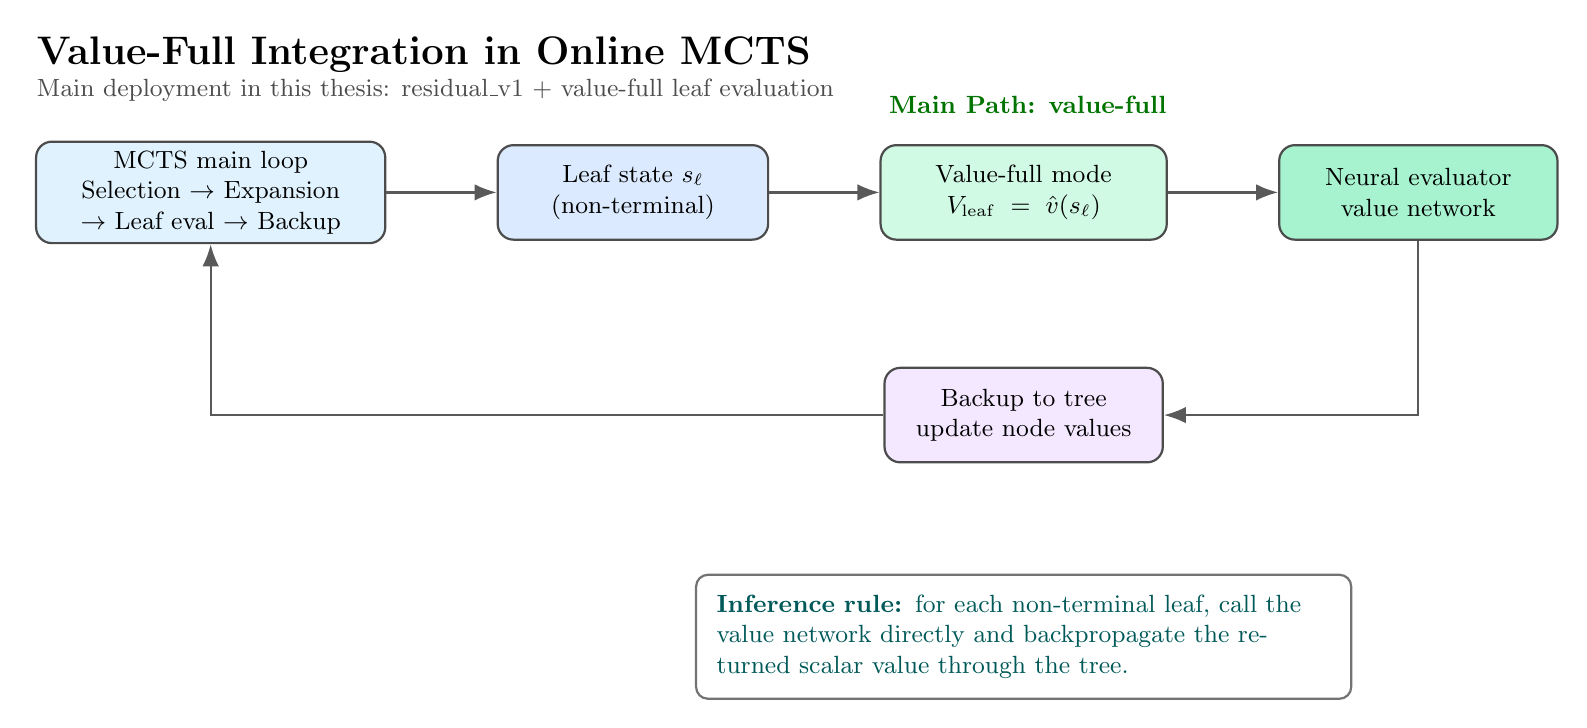
\begin{tikzpicture}[
    font=\small,
    node distance=10mm and 14mm,
    box/.style={draw=black!70, rounded corners=2mm, thick, align=center, minimum height=12mm},
    arr/.style={-{Latex[length=2.8mm]}, thick, draw=black!65},
    note/.style={draw=black!55, rounded corners=1.5mm, thick, align=left, fill=white, inner sep=2.6mm}
]

\node[draw=none, font=\Large\bfseries, anchor=west] at (-0.1,3.95) {Value-Full Integration in Online MCTS};
\node[draw=none, font=\small, text=black!70, anchor=west] at (-0.1,3.50) {Main deployment in this thesis: residual\_v1 + value-full leaf evaluation};

\node[box, fill=cLoop, text width=42mm, anchor=west] (loop) at (0,2.20) {MCTS main loop\\Selection $\rightarrow$ Expansion\\$\rightarrow$ Leaf eval $\rightarrow$ Backup};
\node[box, fill=cLeaf, text width=32mm, right=of loop] (leaf) {Leaf state $s_\ell$\\(non-terminal)};
\node[box, fill=cValue, text width=34mm, right=of leaf] (value) {Value-full mode\\$V_{\mathrm{leaf}}=\hat{v}(s_\ell)$};
\node[box, fill=cNeural, text width=33mm, right=of value] (neural) {Neural evaluator\\value network};
\node[box, fill=cBackup, text width=33mm, below=16mm of value] (backup) {Backup to tree\\update node values};

\draw[arr] (loop.east) -- (leaf.west);
\draw[arr] (leaf.east) -- (value.west);
\draw[arr] (value.east) -- (neural.west);
\draw[arr] (neural.south) |- (backup.east);
\draw[arr] (backup.west) -| (loop.south);

\node[note, text width=78mm, text=teal!70!black, below=14mm of backup] (note1) {\textbf{Inference rule:} for each non-terminal leaf, call the value network directly and backpropagate the returned scalar value through the tree.};
\node[draw=none, font=\bfseries\small, text=green!45!black, anchor=west] at ($(value.north west)+(0mm,5mm)$) {Main Path: value-full};

\end{tikzpicture}
\end{document}
